\documentclass{article}
\usepackage[utf8]{inputenc}
\usepackage[portuges]{babel}
\usepackage{csquotes}
\usepackage{geometry}
\usepackage{indentfirst}
\usepackage{graphicx}
\usepackage{float}
\usepackage[backend = biber]{biblatex}
\addbibresource{referencias.bib}
\geometry{top = 3cm, bottom = 2cm, left = 3cm, right = 2cm}

\title{Banco de Dados}
\author{Anne Beatriz Cardoso \\ Igor Cortes Junqueira \\ Igor Patrício Michels \\ João Vinícius Primaki Prado}
\date{2020.2}

\begin{document}

\maketitle

\section{Introdução}

O presente documento tem por objetivo relatar o desenvolvimento da elaboração de um banco de dados para a primeira avaliação da disciplina de Banco de Dados da FGV-EMAp, ministrada pelo professor Renato Rocha Souza. O objetivo inicial era a criação de um banco de dados sobre o tema comida, entretanto, após algumas conversas entre o grupo e autorização do professor, trocou-se para a elaboração de um banco de dados com informações sobre os voos domésticos dos EUA entre janeiro de 2019 e maio de 2020. A escolha por tal período foi feita para possibilitar comparações do pré e pós pandemia nos EUA.

\section{Elaboração}

\subsection{Fontes}

Os dados dos voos utilizados foram obtidos por meio dos registros oficiais da BTS - Bureau of Transportation Statistics \cite{BTS}, já os dados das aeronaves foram obtidos pelos registros da FAA - Federal Aviation Administration \cite{FAA}.

\subsection{Extração dos dados}

Para a extração dos dados da BTS simplesmente acessamos o site e baixamos os dados completos, mês a mês, de janeiro 2019 a maio de 2020\footnote{O site não possuía registros mais recentes.}, feito isso, obtivemos um total de 3,26 GB de registros, tudo em 17 arquivos csv.
\begin{figure}[H]
    \centering
    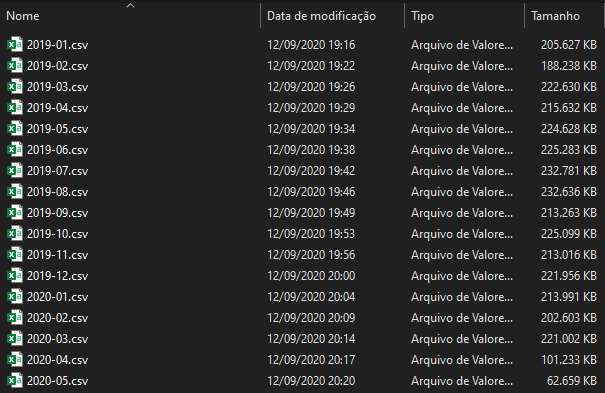
\includegraphics[scale = 0.5]{Imagens/Arquivos.png}
    \caption{Print dos arquivos}
    \label{fig: print}
\end{figure}

Após isso, precisamos buscar os dados das aeronaves. Assim, pelos registros dos voos pegamos os registros de cada aeronave utilizada e buscamos os respectivos registros no site da FAA.

Como a FAA não libera um arquivo com os dados das aeronaves, foi elaborado um script para fazer a busca e coleta dos dados das aeronaves utilizadas. Para fazer tal script também foi elaborado um arquivo .txt com todos os registros de aeronaves encontrados nos registros da BTS.

Durante a execução desse script ocorreram alguns erros de leitura, pois nem todas as aeronaves possuiam registro ativo na FAA, então criamos uma lista de ``falhas''. Houveram, de um total de 5998 aeronaves, 70 com falha na coleta\footnote{Aeronaves sem registro ou sem registro ativo.}. Dessas falhas, reformulamos o script e o executamos novamente ele para realizar a coleta dos dados, dessa forma conseguimos coletar os dados de 40 aeronaves com registro vencido, as outras 30 não possuiam registro na FAA, então ficaram sem dados de fabricante, companhia, etc.

A saída desse script foi dada pela geração de 6 arquivos csv, cada um correspondendo a uma tabela do banco (aircraft\_model, aircraft\_types, aircrafts, companies, engine\_types e manufacturers).

\subsection{Manipulação}




\section{Resultados}

Um primeiro resultado interessante já pôde ser observado na figura \ref{fig: print}. Lá pudemos ver, na última coluna, que o tamanho dos arquivos diminuiu muito nos meses de abril e maio de 2020 quando comparado aos demais meses, em especial no mesmo período de 2019, ou seja, os estadunidenses passaram a viajar menos e, com isso, o arquivo passou a ter menos dados. Isso já se mostrou ser um dos reflexos do coronavírus, uma vez que a população passou a ficar mais isolada.



\printbibliography

\end{document}
